% ******************************* PhD Thesis Template **************************
% Please have a look at the README.md file for info on how to use the template

\documentclass[a4paper,PageStyleII, 12pt,times,numbered,print,custommargin,index,tufte-handout]{PhDThesisPSnPDF}
\usepackage[romanian]{babel}

\renewcommand{\thefigure}{\arabic{chapter}.\arabic{figure}}
\renewcommand{\thetable}{\arabic{chapter}.\arabic{table}}
\renewcommand{\theequation}{\arabic{chapter}.\arabic{equation}}

\usepackage[tablename=Tabel]{caption}
% ******************************************************************************
% ******************************* Class Options ********************************
% *********************** See README for more details **************************
% ******************************************************************************

% `a4paper
% `11pt' or `12pt'(default)
%
% `oneside' or `twoside'(default): Printing double side (twoside) or single
% side.
%
% `print': Use `print' for print version with appropriate margins and page
% layout. Leaving the options field blank will activate Online version.
%
% `index': For index at the end of the thesis
%
% `draftclassic': For draft mode without loading any images (same as draft in book)
%
% `draft': Special draft mode with line numbers, images, and water mark with
% timestamp and custom text. Position of the text can also be modified.
%
% `abstract': To generate only the title page and abstract page with
% dissertation title and name, to submit to the Student Registry
%
% `chapter`: This option enables only the specified chapter and it's references
%  Useful for review and corrections.
%
% ************************* Custom Page Margins ********************************
%
% `custommargin`: Use `custommargin' in options to activate custom page margins,
% which can be defined in the preamble.tex. Custom margin will override
% print/online margin setup.
%
% *********************** Choosing the Fonts in Class Options ******************
%
% `times' : Times font with math support.
%
% `fourier': Utopia Font with Fourier Math font (Font has to be installed)
%            It's a free font.
%
% `customfont': Use `customfont' option in the document class and load the
% package in the preamble.tex
%
% default or leave empty: `Latin Modern' font will be loaded.
%
% ********************** Choosing the Bibliography style ***********************
%
% `authoryear': For author-year citation eg., Krishna (2013)
%
% `numbered': (Default Option) For numbered and sorted citation e.g., [1,5,2]
%
% `custombib': Define your own bibliography style in the `preamble.tex' file.
%              `\RequirePackage[square, sort, numbers, authoryear]{natbib}'.
%              This can be also used to load biblatex instead of natbib
%              (See Preamble)
%
% **************************** Choosing the Page Style *************************
%
% `default (leave empty)': For Page Numbers in Header (Left Even, Right Odd) and
% Chapter Name in Header (Right Even) and Section Name (Left Odd). Blank Footer.
%
% `PageStyleI': Chapter Name next & Page Number on Even Side (Left Even).
% Section Name & Page Number in Header on Odd Side (Right Odd). Footer is empty.
%
% `PageStyleII': Chapter Name on Even Side (Left Even) in Header. Section Number
% and Section Name in Header on Odd Side (Right Odd). Page numbering in footer
% ********************************** Preamble **********************************
% Preamble: Contains packages and user-defined commands and settings
% ******************************************************************************
% ****************************** Custom Margin *********************************

% Add `custommargin' in the document class options to use this section
% Set {innerside margin / outerside margin / topmargin / bottom margin}  and
% other page dimensions
\ifsetCustomMargin
  \RequirePackage[left=1.5in,right=1in,top=1in,bottom=1in]{geometry}
  \setFancyHdr % To apply fancy header after geometry package is loaded
\fi

% Add spaces between paragraphs
%\setlength{\parskip}{0.5em}
% Ragged bottom avoids extra whitespaces between paragraphs
\raggedbottom
% To remove the excess top spacing for enumeration, list and description
%\usepackage{enumitem}
%\setlist[enumerate,itemize,description]{topsep=0em}

% *****************************************************************************
% ******************* Fonts (like different typewriter fonts etc.)*************

% Add `customfont' in the document class option to use this section

\ifsetCustomFont
  % Set your custom font here and use `customfont' in options. Leave empty to
  % load computer modern font (default LaTeX font).
  %\RequirePackage{helvet}

  % For use with XeLaTeX
  %  \setmainfont[
  %    Path              = ./libertine/opentype/,
  %    Extension         = .otf,
  %    UprightFont = LinLibertine_R,
  %    BoldFont = LinLibertine_RZ, % Linux Libertine O Regular Semibold
  %    ItalicFont = LinLibertine_RI,
  %    BoldItalicFont = LinLibertine_RZI, % Linux Libertine O Regular Semibold Italic
  %  ]
  %  {libertine}
  %  % load font from system font
  %  \newfontfamily\libertinesystemfont{Linux Libertine O}
\fi

% *****************************************************************************
% **************************** Custom Packages ********************************

% ************************* Algorithms and Pseudocode **************************

%\usepackage{algpseudocode}


% ********************Captions and Hyperreferencing / URL **********************

% Captions: This makes captions of figures use a boldfaced small font.
%\RequirePackage[small,bf]{caption}

\RequirePackage[labelsep=space,tableposition=top]{caption}
\renewcommand{\figurename}{Fig.} %to support older versions of captions.sty


% *************************** Graphics and figures *****************************

%\usepackage{rotating}
%\usepackage{wrapfig}

% Uncomment the following two lines to force Latex to place the figure.
% Use [H] when including graphics. Note 'H' instead of 'h'
%\usepackage{float}
%\restylefloat{figure}

% Subcaption package is also available in the sty folder you can use that by
% uncommenting the following line
% This is for people stuck with older versions of texlive
%\usepackage{sty/caption/subcaption}
\usepackage{subcaption}

% ********************************** Tables ************************************
\usepackage{booktabs} % For professional looking tables
\usepackage{multirow}

%\usepackage{multicol}
%\usepackage{longtable}
%\usepackage{tabularx}


% *********************************** SI Units *********************************
\usepackage{siunitx} % use this package module for SI units


% ******************************* Line Spacing *********************************

% Choose linespacing as appropriate. Default is one-half line spacing as per the
% University guidelines

% \doublespacing
% \onehalfspacing
% \singlespacing


% ************************ Formatting / Footnote *******************************

% Don't break enumeration (etc.) across pages in an ugly manner (default 10000)
%\clubpenalty=500
%\widowpenalty=500

%\usepackage[perpage]{footmisc} %Range of footnote options


% *****************************************************************************
% *************************** Bibliography  and References ********************

%\usepackage{cleveref} %Referencing without need to explicitly state fig /table

% Add `custombib' in the document class option to use this section
\ifuseCustomBib
   \RequirePackage[square, sort, numbers, authoryear]{natbib} % CustomBib

% If you would like to use biblatex for your reference management, as opposed to the default `natbibpackage` pass the option `custombib` in the document class. Comment out the previous line to make sure you don't load the natbib package. Uncomment the following lines and specify the location of references.bib file

%\RequirePackage[backend=biber, style=numeric-comp, citestyle=numeric, sorting=nty, natbib=true]{biblatex}
%\addbibresource{References/references} %Location of references.bib only for biblatex, Do not omit the .bib extension from the filename.

\fi

% changes the default name `Bibliography` -> `References'
\renewcommand{\bibname}{References}


% ******************************************************************************
% ************************* User Defined Commands ******************************
% ******************************************************************************

% *********** To change the name of Table of Contents / LOF and LOT ************

%\renewcommand{\contentsname}{My Table of Contents}
%\renewcommand{\listfigurename}{My List of Figures}
%\renewcommand{\listtablename}{My List of Tables}


% ********************** TOC depth and numbering depth *************************

\setcounter{secnumdepth}{2}
\setcounter{tocdepth}{2}


% ******************************* Nomenclature *********************************

% To change the name of the Nomenclature section, uncomment the following line

%\renewcommand{\nomname}{Symbols}


% ********************************* Appendix ***********************************

% The default value of both \appendixtocname and \appendixpagename is `Appendices'. These names can all be changed via:

%\renewcommand{\appendixtocname}{List of appendices}
%\renewcommand{\appendixname}{Appndx}

% *********************** Configure Draft Mode **********************************

% Uncomment to disable figures in `draft'
%\setkeys{Gin}{draft=true}  % set draft to false to enable figures in `draft'

% These options are active only during the draft mode
% Default text is "Draft"
%\SetDraftText{DRAFT}

% Default Watermark location is top. Location (top/bottom)
%\SetDraftWMPosition{bottom}

% Draft Version - default is v1.0
%\SetDraftVersion{v1.1}

% Draft Text grayscale value (should be between 0-black and 1-white)
% Default value is 0.75
%\SetDraftGrayScale{0.8}


% ******************************** Todo Notes **********************************
%% Uncomment the following lines to have todonotes.

%\ifsetDraft
%	\usepackage[colorinlistoftodos]{todonotes}
%	\newcommand{\mynote}[1]{\todo[author=kks32,size=\small,inline,color=green!40]{#1}}
%\else
%	\newcommand{\mynote}[1]{}
%	\newcommand{\listoftodos}{}
%\fi

% Example todo: \mynote{Hey! I have a note}

% ******************************** Highlighting Changes **********************************
%% Uncomment the following lines to be able to highlight text/modifications.
%\ifsetDraft
%  \usepackage{color, soul}
%  \newcommand{\hlc}[2][yellow]{{\sethlcolor{#1} \hl{#2}}}
%  \newcommand{\hlfix}[2]{\texthl{#1}\todo{#2}}
%\else
%  \newcommand{\hlc}[2]{}
%  \newcommand{\hlfix}[2]{}
%\fi

% Example highlight 1: \hlc{Text to be highlighted}
% Example highlight 2: \hlc[green]{Text to be highlighted in green colour}
% Example highlight 3: \hlfix{Original Text}{Fixed Text}

% *****************************************************************************
% ******************* Better enumeration my MB*************
\usepackage{enumitem}


% ************************ Thesis Information & Meta-data **********************
% Thesis title and author information, refernce file for biblatex
% ************************ Thesis Information & Meta-data **********************
%% The title of the thesis
\title{Tez\u{a} de doctorat}
%\texorpdfstring is used for PDF metadata. Usage:
%\texorpdfstring{LaTeX_Version}{PDF Version (non-latex)} eg.,
%\texorpdfstring{$sigma$}{sigma}

%% The full name of the author
\author{Ing. Georgian Iosef, Ing. Adrian-Zamfirel Teșulă}

%% Thesis title both in Romanian and English
\rotitle{Model de redactare a tezei de doctorat la \c{s}coala doctoral\u{a} SD-ETTI}
\entitle{Model for writing the doctoral thesis at SD-ETTI Doctoral School}

%% Doctoral School's name
\doctoralschool{\c{S}coala Doctoral\u{a} de Electronic\u{a}, Telecomunica\c{t}ii \c{s}i Tehnologia Informa\c{t}iei }

%% University name
\university{Universitatea Politehnica din Bucure\c{s}ti}

%% Decision number and date
\decisionnumber{XXX}
\decisiondate{DD-MM-YYYY}

%% Doctoral comitte title
\doctoralcommitteetitle{Comisia de doctorat}

%% Doctoral comitte table
\doctoralcommitteetable{
\textbf{Prof. Dr. Ing. Bogdan IONESCU}              & \multirow{2}{*}{Pre\c{s}edinte}             \\[-3pt]
Univ. Politehnica din Bucure\c{s}ti                           &                                         \\ 
\textbf{Prof. Dr. Ing. Gheorghe BREZEANU}           & \multirow{2}{*}{Conduc\u{a}tor de doctorat} \\[-3pt]
Univ. Politehnica din Bucure\c{s}ti                           &                                         \\ 
\textbf{Prof. Dr. Ing. Ion MARGHESCU}               & \multirow{2}{*}{Referent}                   \\[-3pt]
Univ. Politehnica din Bucure\c{s}ti                           &                                         \\ 
\textbf{Prof. Dr. Ing. Mihai CIUC}                  & \multirow{2}{*}{Referent}                   \\[-3pt]
Univ. Politehnica din Bucure\c{s}ti                           &                                         \\ 
\textbf{Dr. Ing. Dorin COM\u{A}NICIU}               & \multirow{2}{*}{Referent}                   \\[-3pt]
Siemens Healthcare                                  &                                                  \\ 
}

%% Submission date
% Default is set as {\monthname[\the\month]\space\the\year}
\degreedate{BUCURE\c{S}TI 2021} 

%% Meta information
\subject{LaTeX} \keywords{{LaTeX} {PhD Thesis} {SD-ETTI} {University Politehnica of Bucharest}}

% ***************************** Abstract Separate ******************************
% To printout only the titlepage and the abstract with the PhD title and the
% author name for submission to the Student Registry, use the `abstract' option in
% the document class.

\ifdefineAbstract
 \pagestyle{empty}
 \includeonly{Declaration/declaration, Abstract/abstract}
\fi

% ***************************** Chapter Mode ***********************************
% The chapter mode allows user to only print particular chapters with references
% Title, Contents, Frontmatter are disabled by default
% Useful option to review a particular chapter or to send it to supervisior.
% To use choose `chapter' option in the document class

\ifdefineChapter
 \includeonly{Chapter3/chapter3}
\fi

% ******************************** Front Matter ********************************
\begin{document}

\frontmatter

\maketitle
%!TEX root = ../thesis.tex
%*******************************************************************************
%******************************* Instructions **********************************
%*******************************************************************************

\ifpdf
    \graphicspath{{Instructions/Figs/Raster/}{Instructions/Figs/PDF/}{Instructions/Figs/}}
\else
    \graphicspath{{Instructions/Figs/Vector/}{Instructions/Figs/}}
\else
    \graphicspath{{Instructions/Figs/Regular/}{Instructions/Regular/}}    
\fi

\thispagestyle{empty}
 \newpage
 \newpage
\begin{center}
\section*{Instruc\c{t}iuni de redactare pentru doctoranzi}
\vspace{-0.5cm}
(\textcolor{red}{acest text nu face parte din tez\u{a}})
\end{center}

\thispagestyle{empty}
\subsection*{Instruc\c{t}iuni de formatare generale}
\begin{itemize}
  \item Teza se redacteaz\u{a} \^{i}n format A4, la 1,15 r\^{a}nduri, cu caractere Times New Roman de 12pt. \c{s}i diacritice. Tip\u{a}rirea se face pe ambele fe\c{t}e ale foii A4.
  \item Marginile textului sunt la 1,5$''$ (3,5 cm) st\^{a}nga \c{s}i 1$''$ (2,5 cm) dreapta, sus \c{s}i jos. Num\u{a}rul paginii se insereaz\u{a} jos, central, la cel pu\c{t}in 0,75$''$ (2 cm) de marginea de jos a paginii. Coperta interioar\u{a} nu se pagineaz\u{a}.
  \item Paginile de: Mul\c{t}tumiri, Cuprins, Lista tabelelor, Lista figurilor şi Lista abrevierilor se pagineaz\u{a} cu cifre romane mici: i, ii, iii, etc.
  \item Capitolele, bibliografia \c{s}i anexele se pagineaz\u{a} cu cifre arabe. Excep\c{t}ie face prima pagin\u{a} a fiec\u{a}rui capitol, pe care num\u{a}rul paginii nu trebuie să apar\u{a}.
  \item Paginile pare ale capitolelor au în antet titlul tezei scris cu caractere Times New Roman de 10pt. La nevoie, titlul trebuie prescurtat astfel \^{i}nc\^{a}t s\u{a} \^{i}ncap\u{a} pe un singur r\^{a}nd.
  \item Paginile impare ale capitolelor au \^{i}n antet titlul capitolului scris cu caractere Times New Roman de 10pt. Excep\c{t}ie face prima pagin\u{a} a fiec\u{a}rui capitol.
  \item Teza cuprinde, \^{i}n ordine, urm\u{a}toarele sec\c{t}iuni/informa\c{t}ii:
  \begin{itemize}
  \item Coperta interioar\u{a} (pagina din dreapta).
  \item Pagina liber\u{a} (verso-ul coper\c{t}ii).
  \item Pagina de mul\c{t}umiri.
  \item Cuprins.
  \item Lista tabelelor.
  \item Lista figurilor.
  \item Lista abrevierilor.
  \item Capitolele tezei.
  \item Anexe.
  \item Bibliografie.
  \end{itemize}
  \item Toate sec\c{t}iunile \^{i}ncep pe pagin\u{a} impar\u{a} (pagina din dreapta \^{i}n varianta tip\u{a}rit\u{a}). 
  \item Trebuie evitat\u{a} terminarea textului prin linii izolate în partea de sus a unei pagini sau scrierea titlului de sec\c{t}iune \^{i}n \^{i}ncheierea unei pagini. 
  \end{itemize}
 
 \thispagestyle{empty}  
\subsection*{Instruc\c{t}iuni pentru Mul\c{t}umiri}
\begin{itemize}
  \item Titlul se scrie pe primul r\^{a}nd, centrat, bold, cu Times New Roman de 18pt. Textul \^{i}ncepe la 2 r\^{a}nduri sub titlu. Textul \^{i}ncepe cu alineat zero. \^{I}n interiorul sec\c{t}iunii, alineatul este la 0,25$''$.
  \end{itemize}
  
\subsection*{Instruc\c{t}iuni pentru Cuprins}
\begin{itemize}
  \item Cuprinde lista tuturor capitolelor, sec\c{t}iunilor (n.1) \c{s}i sub-sec\c{t}iunilor (n.1.1).
\end{itemize}  

\subsection*{Instruc\c{t}iuni pentru Lista tabelelor, Lista figurilor \c{s}i Lista abrevierilor}
\begin{itemize}
  \item Fiecare list\u{a} \^{i}ncepe pe o pagin\u{a} nou\u{a} impar\u{a} (pagina din dreapta în versiunea tip\u{a}rit\u{a}). Titlul listei se scrie la st\^{a}nga, cu caractere bold, Times New Roman de 28pt., la 9 r\^{a}nduri de marginea de sus. Tabelele \c{s}i figurile apar cu numerotarea din capitole. Lista \^{i}ncepe la 3 r\^{a}nduri sub titlu.
\end{itemize} 


\subsection*{Instruc\c{t}iuni pentru Introducere, Concluzii, Capitole \c{s}i Anexe}
\begin{itemize}
  \item Introducerea, concluziile \c{s}i restul capitolelor \^{i}ncep pe o pagin\u{a} nou\u{a} impar\u{a} (pagina din dreapta \^{i}n versiunea tip\u{a}rit\u{a}). Pagina de \^{i}nceput cuprinde:
\begin{itemize}
  \item Capitolul n (st\^{a}nga, bold, Times New Roman de 28pt., la 9 r\^{a}nduri de marginea de sus).
  \item Titlul capitolului (st\^{a}nga, bold, Times New Roman de 28pt., la 2 r\^{a}nduri).
  \item Textul capitolului (Times New Roman de 12pt. la 3 r\^{a}nduri).
  \end{itemize}
  \item Titlul sec\c{t}iunilor (st\^{a}nga, bold, Times New Roman de 18pt., la 2 r\^{a}nduri).
  \item Titlul sub-sec\c{t}iunilor (st\^{a}nga, bold, Times New Roman de 14pt., la 2 r\^{a}nduri).
  \item Textul \^{i}ncepe la 3 r\^{a}nduri sub titlu capitolului \c{s}i la 2 r\^{a}nduri sub titlul sec\c{t}iunii/sub-sec\c{t}iunii, cu alineat zero. \^{i}n interiorul capitolului, alineatul este la 0,25$''$.
  \item Men\c{t}ionarea \^{i}n text a unei referin\c{t}e bibliografice se face cu paranteze drepte. De exemplu [12] face referire la lucrarea cu acest num\u{a}r din Bibliografie.
  \item Capitolul de Introducere trebuie s\u{a} con\c{t}in\u{a} obligatoriu urm\u{a}toarele sec\c{t}iuni:
\begin{itemize}
  \item Prezentarea domeniului tezei de doctorat.
  \item Scopul tezei de doctorat.
  \item Con\c{t}inutul tezei de doctorat.
  \end{itemize}
  \item Capitolul de Concluzii trebuie s\u{a} con\c{t}in\u{a} obligatoriu urm\u{a}toarele sec\c{t}iuni:
\begin{itemize}
  \item Rezultate ob\c{t}inute.
  \item Contribu\c{t}ii originale.
  \item Lista lucr\u{a}rilor originale.
  \item Perspective de dezvoltare ulterioar\u{a}.
  \end{itemize}
  \item Anexele se editeaz\u{a} dup\u{a} regulile pentru capitole. Singura diferen\c{t}\u{a} apare la nivelul primului titlu, care se nume\c{s}te Anexe.
  \end{itemize}
  
\subsection*{Instruc\c{t}iuni pentru ecua\c{t}ii, tabele \c{s}i figuri}
\begin{itemize}
  \item Ecua\c{t}iile trebuie s\u{a} fie centrate \c{s}i numerotate \^{i}n func\c{t}ie de num\u{a}rul capitolului \c{s}i ordinea din capitol. Primul num\u{a}r reprezint\u{a} num\u{a}rul capitolului, iar cel de al doilea num\u{a}rul de ordine al ecua\c{t}iei \^{i}n capitol. Ecua\c{t}iile se scriu cu un editor de ecua\c{t}ii, av\^{a}nd dimensiunea de 12pt. (ca \c{s}i textul). Se vor explica termenii folosiți. Exemplu: 
  \begin{equation}
      E = m\cdot c^{2}
  \end{equation}
  
  unde \textit{E} reprezint\u{a} energia, \textit{m} masa iar \textit{c} este viteza luminii.          
  \item Figurile \c{s}i Tabelele se centreaz\u{a} \c{s}i trebuie s\u{a} aib\u{a} dimensiuni suficient de mari pentru ca informa\c{t}ia con\c{t}inut\u{a} s\u{a} fie lizibil\u{a}. Pentru tabele textul se recomand\u{a} s\u{a} fie Times New Roman \^{i}ntre 9pt. \c{s}i 12pt., nu mai mare dec\^{a}t textul din sec\c{t}iuni. Imaginile, diagramele, prezentate \^{i}n figuri trebuie s\u{a} aib\u{a} o rezolu\c{t}ie suficient de mare pentru ca toate informa\c{t}iile din acestea s\u{a} fie lizibile. Se recomand\u{a} generarea acestora vectorial\u{a}, astfel \^{i}ncât s\u{a} poat\u{a} fi scalabile la vizualizare. Titlul tabelelor \c{s}i legenda figurilor se scriu cu caractere Times New Roman, italic, de 12pt. \c{s}i se numeroteaz\u{a} \^{i}n func\c{t}ie de num\u{a}rul capitolului \c{s}i ordinea \^{i}n capitol. Titlul tabelelor se g\u{a}se\c{s}te \^{i}n partea de sus a tabelului iar legenda figurilor \^{i}n partea de jos a figurii. Este absolut necesar\u{a} referirea la aceste tabele \c{s}i figuri \^{i}n textul tezei unde sunt explicate \c{s}i comentate. Urm\u{a}ri\c{t}i exemplele de formatare de la Figura~\ref{fig:exemplu_figura} \c{s}i Tabel~\ref{tab:exemplu_tabel}.  
    \end{itemize}
 
\thispagestyle{empty}
\begin{table}[hbt!]
\centering
\caption{Date numerice ob\c{t}inute în urma m\u{a}sur\u{a}torilor.}
\label{tab:exemplu_tabel}
\begin{tabular}{|l|l|l|}
\hline
\multicolumn{1}{|c|}{\textbf{Col 1}} & \multicolumn{1}{c|}{\textbf{Col 2}} & \multicolumn{1}{c|}{\textbf{Col 3}} \\ \hline
1.12678                              & 2.12678                             & 3.12678                             \\ \hline
\end{tabular}
\end{table}

\begin{figure}
     \centering
     \begin{subfigure}[b]{0.45\textwidth}
         \centering
         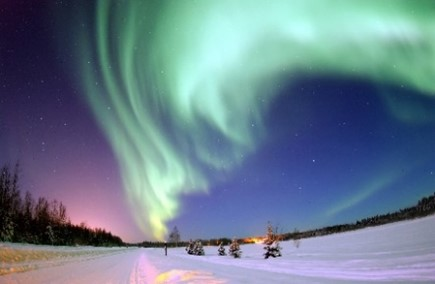
\includegraphics[width=\textwidth]{Instructions/Figs/Regular/Picture1.jpg}
         \caption{}
         \label{fig:a}
     \end{subfigure}
     \hfill
     \begin{subfigure}[b]{0.45\textwidth}
         \centering
         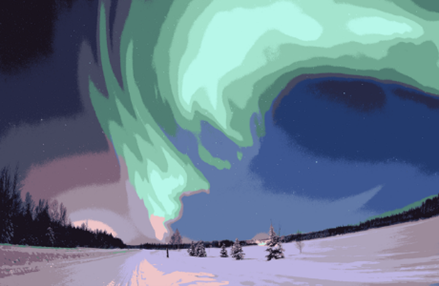
\includegraphics[width=\textwidth]{Instructions/Figs/Regular/Picture2.png}
         \caption{}
         \label{fig:b}
     \end{subfigure}
     \hfill
    \caption{Exemplu de segmentare imagine: (a) imaginea ini\c{t}ial\u{a}, (b) imaginea segmentat\u{a}.}
    \label{fig:exemplu_figura}
\end{figure}
  
\subsection*{Instruc\c{t}iuni pentru Bibliografie}
\begin{itemize}
  \item Referin\c{t}ele bibliografice trebuie plasate la sf\^{a}r\c{s}itul tezei. Este absolut necesar\u{a} referirea la bibliografie \^{i}n textul tezei \c{s}i nu doar listarea referin\c{t}elor bibliografice.
  \item Titlul Bibliografie se scrie cu caractere Times New Roman, bold, de 28pt., la 8 r\^{a}nduri de marginea de sus. Con\c{t}inutul bibliografiei \^{i}ncepe la 2 r\^{a}nduri sub titlu \c{s}i se scrie cu caractere Times New Roman de dimensiune 11pt. O referin\c{t}\u{a} bibliografic\u{a} trebuie s\u{a} con\c{t}in\u{a} toate informa\c{t}iile cu privire la publica\c{t}ie astfel \^{i}nc\^{a}t aceasta s\u{a} fie u\c{s}or identificat\u{a} pentru consultare, exemplu \cite{demarty2014multimodal, duta2017spatio, purica2015multiview}:
\end{itemize}


\noindent
[1] C.-H. Demarty, C. Penet, B. Ionescu, G. Gravier, M. Soleymani, \textit{Multimodal violence detection in Hollywood movies: State-of-the-art and Benchmarking}, Fusion in Computer Vision - Understanding Complex Visual Content, Springer Advances in Computer Vision and Pattern Recognition, pp. 185-208, ISBN: 978-3-319-05695-1, Eds. J. Benois-Pineau, G. Quénot, T. Piatrik, B. Ionescu, 2014.

\noindent
[2] I.C. Duță, B. Ionescu, K. Aizawa, N. Sebe, \textit{Spatio-temporal VLAD Encoding for Human Action Recognition in Videos}, International Conference on Multimedia Modeling - MMM, pp. 365-378, January 4-6, Reykjavík, Iceland, 2017.

\noindent
[3] A.I. Purică, E.G. Mora, B. Pesquet-Popescu, M. Cagnazzo, B. Ionescu, \textit{Multiview plus Depth Video Coding with Temporal Prediction View Synthesis}, IEEE Transactions on Circuits and Systems for Video Technology, 26(2), pp. 360-374, 2016.

\subsection*{Instruc\c{t}iuni \LaTeX}

Instruc\c{t}iunile \LaTeX~se reg\u{a}sesc \^{i}n fi\c{s}ierul README.md.
\thispagestyle{empty}
% ************************** Thesis Acknowledgements **************************

\begin{acknowledgements}      


Lorem ipsum dolor sit amet, consectetur adipiscing elit, sed do eiusmod tempor incididunt ut labore et dolore magna aliqua. Facilisi morbi tempus iaculis urna id volutpat lacus laoreet non. Arcu non sodales neque sodales ut etiam sit. Nascetur ridiculus mus mauris vitae ultricies leo integer malesuada nunc. Nulla aliquet enim tortor at auctor urna. Placerat orci nulla pellentesque dignissim enim sit. Est ullamcorper eget nulla facilisi. Vitae congue mauris rhoncus aenean vel elit scelerisque mauris. Nisl vel pretium lectus quam id leo in vitae turpis. Ac ut consequat semper viverra nam libero justo laoreet. Quis ipsum suspendisse ultrices gravida dictum fusce ut placerat orci. In iaculis nunc sed augue lacus viverra vitae. Feugiat nibh sed pulvinar proin. Venenatis cras sed felis eget. Egestas integer eget aliquet nibh. Non arcu risus quis varius. Sed sed risus pretium quam vulputate.

Est ultricies integer quis auctor elit sed vulputate mi sit. Etiam sit amet nisl purus in mollis nunc sed. Nunc pulvinar sapien et ligula ullamcorper malesuada proin libero. Fermentum leo vel orci porta non pulvinar neque laoreet suspendisse. Donec ultrices tincidunt arcu non sodales. In iaculis nunc sed augue lacus viverra vitae congue eu. Vitae purus faucibus ornare suspendisse sed nisi. Condimentum lacinia quis vel eros donec ac odio. Aliquam nulla facilisi cras fermentum odio eu feugiat pretium. Et ligula ullamcorper malesuada proin libero nunc consequat interdum. Hendrerit dolor magna eget est lorem ipsum dolor sit amet. Scelerisque in dictum non consectetur. Neque viverra justo nec ultrices dui sapien. Semper risus in hendrerit gravida rutrum quisque. Ut ornare lectus sit amet. Aliquet nec ullamcorper sit amet risus nullam eget. Dignissim diam quis enim lobortis scelerisque fermentum.     


\end{acknowledgements}

\include{Abstract/abstract}

% *********************** Adding TOC and List of Figures ***********************

\tableofcontents

\listoftables

\listoffigures

% \printnomenclature[space] space can be set as 2em between symbol and description
%\printnomenclature[3em]

\printnomenclature

% ******************************** Main Matter *********************************
\mainmatter

% Remove page numbers from first page of chapters
\makeatletter
\renewcommand\chapter{\if@openright\cleardoublepage\else\clearpage\fi
                    \thispagestyle{empty}% original style: plain
                    \global\@topnum\z@
                    \@afterindentfalse
                    \secdef\@chapter\@schapter}
\makeatother

%!TEX root = ../thesis.tex
%*******************************************************************************
%*********************************** First Chapter *****************************
%*******************************************************************************

\chapter{Introducere}  %Title of the First Chapter

\ifpdf
    \graphicspath{{Chapter1/Figs/Raster/}{Chapter1/Figs/PDF/}{Chapter1/Figs/}}
\else
    \graphicspath{{Chapter1/Figs/Vector/}{Chapter1/Figs/}}
\fi

Lorem ipsum dolor sit amet, consectetur adipiscing elit, sed do eiusmod tempor incididunt ut labore et dolore magna aliqua. Facilisi morbi tempus iaculis urna id volutpat lacus laoreet non. Arcu non sodales neque sodales ut etiam sit. Nascetur ridiculus mus mauris vitae ultricies leo integer malesuada nunc. Nulla aliquet enim tortor at auctor urna. Placerat orci nulla pellentesque dignissim enim sit. Est ullamcorper eget nulla facilisi. Vitae congue mauris rhoncus aenean vel elit scelerisque mauris. Nisl vel pretium lectus quam id leo in vitae turpis. Ac ut consequat semper viverra nam libero justo laoreet. Quis ipsum suspendisse ultrices gravida dictum fusce ut placerat orci. In iaculis nunc sed augue lacus viverra vitae. Feugiat nibh sed pulvinar proin. Venenatis cras sed felis eget. Egestas integer eget aliquet nibh. Non arcu risus quis varius. Sed sed risus pretium quam vulputate.
Est ultricies integer quis auctor elit sed vulputate mi sit. Etiam sit amet nisl purus in mollis nunc sed. Nunc pulvinar sapien et ligula ullamcorper malesuada proin libero. Fermentum leo vel orci porta non pulvinar neque laoreet suspendisse. Donec ultrices tincidunt arcu non sodales. In iaculis nunc sed augue lacus viverra vitae congue eu. Vitae purus faucibus ornare suspendisse sed nisi. Condimentum lacinia quis vel eros donec ac odio. Aliquam nulla facilisi cras fermentum odio eu feugiat pretium. Et ligula ullamcorper malesuada proin libero nunc consequat interdum. Hendrerit dolor magna eget est lorem ipsum dolor sit amet. Scelerisque in dictum non consectetur. Neque viverra justo nec ultrices dui sapien. Semper risus in hendrerit gravida rutrum quisque. Ut ornare lectus sit amet. Aliquet nec ullamcorper sit amet risus nullam eget. Dignissim diam quis enim lobortis scelerisque fermentum.


%********************************** %First Section  **************************************
\section{Prezentarea domeniului tezei de doctorat} %Section - 1.1 

Lorem ipsum dolor sit amet, consectetur adipiscing elit, sed do eiusmod tempor incididunt ut labore et dolore magna aliqua. Facilisi morbi tempus iaculis urna id volutpat lacus laoreet non. Arcu non sodales neque sodales ut etiam sit. Nascetur ridiculus mus mauris vitae ultricies leo integer malesuada nunc. Nulla aliquet enim tortor at auctor urna. Placerat orci nulla pellentesque dignissim enim sit. Est ullamcorper eget nulla facilisi. Vitae congue mauris rhoncus aenean vel elit scelerisque mauris. Nisl vel pretium lectus quam id leo in vitae turpis. Ac ut consequat semper viverra nam libero justo laoreet. Quis ipsum suspendisse ultrices gravida dictum fusce ut placerat orci. In iaculis nunc sed augue lacus viverra vitae. Feugiat nibh sed pulvinar proin. Venenatis cras sed felis eget. Egestas integer eget aliquet nibh. Non arcu risus quis varius. Sed sed risus pretium quam vulputate.
Est ultricies integer quis auctor elit sed vulputate mi sit. Etiam sit amet nisl purus in mollis nunc sed. Nunc pulvinar sapien et ligula ullamcorper malesuada proin libero. Fermentum leo vel orci porta non pulvinar neque laoreet suspendisse. Donec ultrices tincidunt arcu non sodales. In iaculis nunc sed augue lacus viverra vitae congue eu. Vitae purus faucibus ornare suspendisse sed nisi. Condimentum lacinia quis vel eros donec ac odio. Aliquam nulla facilisi cras fermentum odio eu feugiat pretium. Et ligula ullamcorper malesuada proin libero nunc consequat interdum. Hendrerit dolor magna eget est lorem ipsum dolor sit amet. Scelerisque in dictum non consectetur. Neque viverra justo nec ultrices dui sapien. Semper risus in hendrerit gravida rutrum quisque. Ut ornare lectus sit amet. Aliquet nec ullamcorper sit amet risus nullam eget. Dignissim diam quis enim lobortis scelerisque fermentum.

%********************************** %Second Section  *************************************
\section{Scopul tezei de doctorat} %Section - 1.2


Lorem ipsum dolor sit amet, consectetur adipiscing elit, sed do eiusmod tempor incididunt ut labore et dolore magna aliqua. Facilisi morbi tempus iaculis urna id volutpat lacus laoreet non. Arcu non sodales neque sodales ut etiam sit. Nascetur ridiculus mus mauris vitae ultricies leo integer malesuada nunc. Nulla aliquet enim tortor at auctor urna. Placerat orci nulla pellentesque dignissim enim sit. Est ullamcorper eget nulla facilisi. Vitae congue mauris rhoncus aenean vel elit scelerisque mauris. Nisl vel pretium lectus quam id leo in vitae turpis. Ac ut consequat semper viverra nam libero justo laoreet. Quis ipsum suspendisse ultrices gravida dictum fusce ut placerat orci. In iaculis nunc sed augue lacus viverra vitae. Feugiat nibh sed pulvinar proin. Venenatis cras sed felis eget. Egestas integer eget aliquet nibh. Non arcu risus quis varius. Sed sed risus pretium quam vulputate.
Est ultricies integer quis auctor elit sed vulputate mi sit. Etiam sit amet nisl purus in mollis nunc sed. Nunc pulvinar sapien et ligula ullamcorper malesuada proin libero. Fermentum leo vel orci porta non pulvinar neque laoreet suspendisse. Donec ultrices tincidunt arcu non sodales. In iaculis nunc sed augue lacus viverra vitae congue eu. Vitae purus faucibus ornare suspendisse sed nisi. Condimentum lacinia quis vel eros donec ac odio. Aliquam nulla facilisi cras fermentum odio eu feugiat pretium. Et ligula ullamcorper malesuada proin libero nunc consequat interdum. Hendrerit dolor magna eget est lorem ipsum dolor sit amet. Scelerisque in dictum non consectetur. Neque viverra justo nec ultrices dui sapien. Semper risus in hendrerit gravida rutrum quisque. Ut ornare lectus sit amet. Aliquet nec ullamcorper sit amet risus nullam eget. Dignissim diam quis enim lobortis scelerisque fermentum.


%********************************** % Third Section  *************************************
\section{Con\c{t}inutul tezei de doctorat}  %Section - 1.3 
\label{section1.3}

Lorem ipsum dolor sit amet, consectetur adipiscing elit, sed do eiusmod tempor incididunt ut labore et dolore magna aliqua. Facilisi morbi tempus iaculis urna id volutpat lacus laoreet non. Arcu non sodales neque sodales ut etiam sit. Nascetur ridiculus mus mauris vitae ultricies leo integer malesuada nunc. Nulla aliquet enim tortor at auctor urna. Placerat orci nulla pellentesque dignissim enim sit. Est ullamcorper eget nulla facilisi. Vitae congue mauris rhoncus aenean vel elit scelerisque mauris. Nisl vel pretium lectus quam id leo in vitae turpis. Ac ut consequat semper viverra nam libero justo laoreet. Quis ipsum suspendisse ultrices gravida dictum fusce ut placerat orci. In iaculis nunc sed augue lacus viverra vitae. Feugiat nibh sed pulvinar proin. Venenatis cras sed felis eget. Egestas integer eget aliquet nibh. Non arcu risus quis varius. Sed sed risus pretium quam vulputate.
Est ultricies integer quis auctor elit sed vulputate mi sit. Etiam sit amet nisl purus in mollis nunc sed. Nunc pulvinar sapien et ligula ullamcorper malesuada proin libero. Fermentum leo vel orci porta non pulvinar neque laoreet suspendisse. Donec ultrices tincidunt arcu non sodales. In iaculis nunc sed augue lacus viverra vitae congue eu. Vitae purus faucibus ornare suspendisse sed nisi. Condimentum lacinia quis vel eros donec ac odio. Aliquam nulla facilisi cras fermentum odio eu feugiat pretium. Et ligula ullamcorper malesuada proin libero nunc consequat interdum. Hendrerit dolor magna eget est lorem ipsum dolor sit amet. Scelerisque in dictum non consectetur. Neque viverra justo nec ultrices dui sapien. Semper risus in hendrerit gravida rutrum quisque. Ut ornare lectus sit amet. Aliquet nec ullamcorper sit amet risus nullam eget. Dignissim diam quis enim lobortis scelerisque fermentum.

\nomenclature[z-GPU]{GPU}{Graphics Processing Unit}

%!TEX root = ../thesis.tex
%*******************************************************************************
%****************************** Second Chapter *********************************
%*******************************************************************************

\chapter{Denumire capitol}

\ifpdf
    \graphicspath{{Chapter2/Figs/Raster/}{Chapter2/Figs/PDF/}{Chapter2/Figs/}}
\else
    \graphicspath{{Chapter2/Figs/Vector/}{Chapter2/Figs/}}
\fi

Lorem ipsum dolor sit amet, consectetur adipiscing elit, sed do eiusmod tempor incididunt ut labore et dolore magna aliqua. Facilisi morbi tempus iaculis urna id volutpat lacus laoreet non. Arcu non sodales neque sodales ut etiam sit. Nascetur ridiculus mus mauris vitae ultricies leo integer malesuada nunc. Nulla aliquet enim tortor at auctor urna. Placerat orci nulla pellentesque dignissim enim sit. Est ullamcorper eget nulla facilisi. Vitae congue mauris rhoncus aenean vel elit scelerisque mauris. Nisl vel pretium lectus quam id leo in vitae turpis. Ac ut consequat semper viverra nam libero justo laoreet. Quis ipsum suspendisse ultrices gravida dictum fusce ut placerat orci. In iaculis nunc sed augue lacus viverra vitae. Feugiat nibh sed pulvinar proin. Venenatis cras sed felis eget. Egestas integer eget aliquet nibh. Non arcu risus quis varius. Sed sed risus pretium quam vulputate.
Est ultricies integer quis auctor elit sed vulputate mi sit. Etiam sit amet nisl purus in mollis nunc sed. Nunc pulvinar sapien et ligula ullamcorper malesuada proin libero. Fermentum leo vel orci porta non pulvinar neque laoreet suspendisse. Donec ultrices tincidunt arcu non sodales. In iaculis nunc sed augue lacus viverra vitae congue eu. Vitae purus faucibus ornare suspendisse sed nisi. Condimentum lacinia quis vel eros donec ac odio. Aliquam nulla facilisi cras fermentum odio eu feugiat pretium. Et ligula ullamcorper malesuada proin libero nunc consequat interdum. Hendrerit dolor magna eget est lorem ipsum dolor sit amet. Scelerisque in dictum non consectetur. Neque viverra justo nec ultrices dui sapien. Semper risus in hendrerit gravida rutrum quisque. Ut ornare lectus sit amet. Aliquet nec ullamcorper sit amet risus nullam eget. Dignissim diam quis enim lobortis scelerisque fermentum.


\section{Denumire sec\c{t}iune}

Lorem ipsum dolor sit amet, consectetur adipiscing elit, sed do eiusmod tempor incididunt ut labore et dolore magna aliqua. Facilisi morbi tempus iaculis urna id volutpat lacus laoreet non. Arcu non sodales neque sodales ut etiam sit. Nascetur ridiculus mus mauris vitae ultricies leo integer malesuada nunc. Nulla aliquet enim tortor at auctor urna. Placerat orci nulla pellentesque dignissim enim sit. Est ullamcorper eget nulla facilisi. Vitae congue mauris rhoncus aenean vel elit scelerisque mauris. Nisl vel pretium lectus quam id leo in vitae turpis. Ac ut consequat semper viverra nam libero justo laoreet. Quis ipsum suspendisse ultrices gravida dictum fusce ut placerat orci. In iaculis nunc sed augue lacus viverra vitae. Feugiat nibh sed pulvinar proin. Venenatis cras sed felis eget. Egestas integer eget aliquet nibh. Non arcu risus quis varius. Sed sed risus pretium quam vulputate.
Est ultricies integer quis auctor elit sed vulputate mi sit. Etiam sit amet nisl purus in mollis nunc sed. Nunc pulvinar sapien et ligula ullamcorper malesuada proin libero. Fermentum leo vel orci porta non pulvinar neque laoreet suspendisse. Donec ultrices tincidunt arcu non sodales. In iaculis nunc sed augue lacus viverra vitae congue eu. Vitae purus faucibus ornare suspendisse sed nisi. Condimentum lacinia quis vel eros donec ac odio. Aliquam nulla facilisi cras fermentum odio eu feugiat pretium. Et ligula ullamcorper malesuada proin libero nunc consequat interdum. Hendrerit dolor magna eget est lorem ipsum dolor sit amet. Scelerisque in dictum non consectetur. Neque viverra justo nec ultrices dui sapien. Semper risus in hendrerit gravida rutrum quisque. Ut ornare lectus sit amet. Aliquet nec ullamcorper sit amet risus nullam eget. Dignissim diam quis enim lobortis scelerisque fermentum.


\subsection{Denumire sub-sec\c{t}iune}
Lorem ipsum dolor sit amet, consectetur adipiscing elit, sed do eiusmod tempor incididunt ut labore et dolore magna aliqua. Facilisi morbi tempus iaculis urna id volutpat lacus laoreet non. Arcu non sodales neque sodales ut etiam sit. Nascetur ridiculus mus mauris vitae ultricies leo integer malesuada nunc. Nulla aliquet enim tortor at auctor urna. Placerat orci nulla pellentesque dignissim enim sit. Est ullamcorper eget nulla facilisi. Vitae congue mauris rhoncus aenean vel elit scelerisque mauris. Nisl vel pretium lectus quam id leo in vitae turpis. Ac ut consequat semper viverra nam libero justo laoreet. Quis ipsum suspendisse ultrices gravida dictum fusce ut placerat orci. In iaculis nunc sed augue lacus viverra vitae. Feugiat nibh sed pulvinar proin. Venenatis cras sed felis eget. Egestas integer eget aliquet nibh. Non arcu risus quis varius. Sed sed risus pretium quam vulputate.
Est ultricies integer quis auctor elit sed vulputate mi sit. Etiam sit amet nisl purus in mollis nunc sed. Nunc pulvinar sapien et ligula ullamcorper malesuada proin libero. Fermentum leo vel orci porta non pulvinar neque laoreet suspendisse. Donec ultrices tincidunt arcu non sodales. In iaculis nunc sed augue lacus viverra vitae congue eu. Vitae purus faucibus ornare suspendisse sed nisi. Condimentum lacinia quis vel eros donec ac odio. Aliquam nulla facilisi cras fermentum odio eu feugiat pretium. Et ligula ullamcorper malesuada proin libero nunc consequat interdum. Hendrerit dolor magna eget est lorem ipsum dolor sit amet. Scelerisque in dictum non consectetur. Neque viverra justo nec ultrices dui sapien. Semper risus in hendrerit gravida rutrum quisque. Ut ornare lectus sit amet. Aliquet nec ullamcorper sit amet risus nullam eget. Dignissim diam quis enim lobortis scelerisque fermentum.

\subsection{Denumire sub-sec\c{t}iune}
Lorem ipsum dolor sit amet, consectetur adipiscing elit, sed do eiusmod tempor incididunt ut labore et dolore magna aliqua. Facilisi morbi tempus iaculis urna id volutpat lacus laoreet non. Arcu non sodales neque sodales ut etiam sit. Nascetur ridiculus mus mauris vitae ultricies leo integer malesuada nunc. Nulla aliquet enim tortor at auctor urna. Placerat orci nulla pellentesque dignissim enim sit. Est ullamcorper eget nulla facilisi. Vitae congue mauris rhoncus aenean vel elit scelerisque mauris. Nisl vel pretium lectus quam id leo in vitae turpis. Ac ut consequat semper viverra nam libero justo laoreet. Quis ipsum suspendisse ultrices gravida dictum fusce ut placerat orci. In iaculis nunc sed augue lacus viverra vitae. Feugiat nibh sed pulvinar proin. Venenatis cras sed felis eget. Egestas integer eget aliquet nibh. Non arcu risus quis varius. Sed sed risus pretium quam vulputate.
Est ultricies integer quis auctor elit sed vulputate mi sit. Etiam sit amet nisl purus in mollis nunc sed. Nunc pulvinar sapien et ligula ullamcorper malesuada proin libero. Fermentum leo vel orci porta non pulvinar neque laoreet suspendisse. Donec ultrices tincidunt arcu non sodales. In iaculis nunc sed augue lacus viverra vitae congue eu. Vitae purus faucibus ornare suspendisse sed nisi. Condimentum lacinia quis vel eros donec ac odio. Aliquam nulla facilisi cras fermentum odio eu feugiat pretium. Et ligula ullamcorper malesuada proin libero nunc consequat interdum. Hendrerit dolor magna eget est lorem ipsum dolor sit amet. Scelerisque in dictum non consectetur. Neque viverra justo nec ultrices dui sapien. Semper risus in hendrerit gravida rutrum quisque. Ut ornare lectus sit amet. Aliquet nec ullamcorper sit amet risus nullam eget. Dignissim diam quis enim lobortis scelerisque fermentum

\section{Denumire sec\c{t}iune}
Lorem ipsum dolor sit amet, consectetur adipiscing elit, sed do eiusmod tempor incididunt ut labore et dolore magna aliqua. Facilisi morbi tempus iaculis urna id volutpat lacus laoreet non. Arcu non sodales neque sodales ut etiam sit. Nascetur ridiculus mus mauris vitae ultricies leo integer malesuada nunc. Nulla aliquet enim tortor at auctor urna. Placerat orci nulla pellentesque dignissim enim sit. Est ullamcorper eget nulla facilisi. Vitae congue mauris rhoncus aenean vel elit scelerisque mauris. Nisl vel pretium lectus quam id leo in vitae turpis. Ac ut consequat semper viverra nam libero justo laoreet. Quis ipsum suspendisse ultrices gravida dictum fusce ut placerat orci. In iaculis nunc sed augue lacus viverra vitae. Feugiat nibh sed pulvinar proin. Venenatis cras sed felis eget. Egestas integer eget aliquet nibh. Non arcu risus quis varius. Sed sed risus pretium quam vulputate.
Est ultricies integer quis auctor elit sed vulputate mi sit. Etiam sit amet nisl purus in mollis nunc sed. Nunc pulvinar sapien et ligula ullamcorper malesuada proin libero. Fermentum leo vel orci porta non pulvinar neque laoreet suspendisse. Donec ultrices tincidunt arcu non sodales. In iaculis nunc sed augue lacus viverra vitae congue eu. Vitae purus faucibus ornare suspendisse sed nisi. Condimentum lacinia quis vel eros donec ac odio. Aliquam nulla facilisi cras fermentum odio eu feugiat pretium. Et ligula ullamcorper malesuada proin libero nunc consequat interdum. Hendrerit dolor magna eget est lorem ipsum dolor sit amet. Scelerisque in dictum non consectetur. Neque viverra justo nec ultrices dui sapien. Semper risus in hendrerit gravida rutrum quisque. Ut ornare lectus sit amet. Aliquet nec ullamcorper sit amet risus nullam eget. Dignissim diam quis enim lobortis scelerisque fermentum.

\subsection{Denumire sub-sec\c{t}iune}
Lorem ipsum dolor sit amet, consectetur adipiscing elit, sed do eiusmod tempor incididunt ut labore et dolore magna aliqua. Facilisi morbi tempus iaculis urna id volutpat lacus laoreet non. Arcu non sodales neque sodales ut etiam sit. Nascetur ridiculus mus mauris vitae ultricies leo integer malesuada nunc. Nulla aliquet enim tortor at auctor urna. Placerat orci nulla pellentesque dignissim enim sit. Est ullamcorper eget nulla facilisi. Vitae congue mauris rhoncus aenean vel elit scelerisque mauris. Nisl vel pretium lectus quam id leo in vitae turpis. Ac ut consequat semper viverra nam libero justo laoreet. Quis ipsum suspendisse ultrices gravida dictum fusce ut placerat orci. In iaculis nunc sed augue lacus viverra vitae. Feugiat nibh sed pulvinar proin. Venenatis cras sed felis eget. Egestas integer eget aliquet nibh. Non arcu risus quis varius. Sed sed risus pretium quam vulputate.
Est ultricies integer quis auctor elit sed vulputate mi sit. Etiam sit amet nisl purus in mollis nunc sed. Nunc pulvinar sapien et ligula ullamcorper malesuada proin libero. Fermentum leo vel orci porta non pulvinar neque laoreet suspendisse. Donec ultrices tincidunt arcu non sodales. In iaculis nunc sed augue lacus viverra vitae congue eu. Vitae purus faucibus ornare suspendisse sed nisi. Condimentum lacinia quis vel eros donec ac odio. Aliquam nulla facilisi cras fermentum odio eu feugiat pretium. Et ligula ullamcorper malesuada proin libero nunc consequat interdum. Hendrerit dolor magna eget est lorem ipsum dolor sit amet. Scelerisque in dictum non consectetur. Neque viverra justo nec ultrices dui sapien. Semper risus in hendrerit gravida rutrum quisque. Ut ornare lectus sit amet. Aliquet nec ullamcorper sit amet risus nullam eget. Dignissim diam quis enim lobortis scelerisque fermentum.

\subsection{Denumire sub-sec\c{t}iune}
Lorem ipsum dolor sit amet, consectetur adipiscing elit, sed do eiusmod tempor incididunt ut labore et dolore magna aliqua. Facilisi morbi tempus iaculis urna id volutpat lacus laoreet non. Arcu non sodales neque sodales ut etiam sit. Nascetur ridiculus mus mauris vitae ultricies leo integer malesuada nunc. Nulla aliquet enim tortor at auctor urna. Placerat orci nulla pellentesque dignissim enim sit. Est ullamcorper eget nulla facilisi. Vitae congue mauris rhoncus aenean vel elit scelerisque mauris. Nisl vel pretium lectus quam id leo in vitae turpis. Ac ut consequat semper viverra nam libero justo laoreet. Quis ipsum suspendisse ultrices gravida dictum fusce ut placerat orci. In iaculis nunc sed augue lacus viverra vitae. Feugiat nibh sed pulvinar proin. Venenatis cras sed felis eget. Egestas integer eget aliquet nibh. Non arcu risus quis varius. Sed sed risus pretium quam vulputate.
Est ultricies integer quis auctor elit sed vulputate mi sit. Etiam sit amet nisl purus in mollis nunc sed. Nunc pulvinar sapien et ligula ullamcorper malesuada proin libero. Fermentum leo vel orci porta non pulvinar neque laoreet suspendisse. Donec ultrices tincidunt arcu non sodales. In iaculis nunc sed augue lacus viverra vitae congue eu. Vitae purus faucibus ornare suspendisse sed nisi. Condimentum lacinia quis vel eros donec ac odio. Aliquam nulla facilisi cras fermentum odio eu feugiat pretium. Et ligula ullamcorper malesuada proin libero nunc consequat interdum. Hendrerit dolor magna eget est lorem ipsum dolor sit amet. Scelerisque in dictum non consectetur. Neque viverra justo nec ultrices dui sapien. Semper risus in hendrerit gravida rutrum quisque. Ut ornare lectus sit amet. Aliquet nec ullamcorper sit amet risus nullam eget. Dignissim diam quis enim lobortis scelerisque fermentum.
%!TEX root = ../thesis.tex
%*******************************************************************************
%****************************** Third Chapter **********************************
%*******************************************************************************
\chapter{Concluzii}

% **************************** Define Graphics Path **************************
\ifpdf
    \graphicspath{{Chapter3/Figs/Raster/}{Chapter3/Figs/PDF/}{Chapter3/Figs/}}
\else
    \graphicspath{{Chapter3/Figs/Vector/}{Chapter3/Figs/}}
\fi


Lorem ipsum dolor sit amet, consectetur adipiscing elit, sed do eiusmod tempor incididunt ut labore et dolore magna aliqua. Facilisi morbi tempus iaculis urna id volutpat lacus laoreet non. Arcu non sodales neque sodales ut etiam sit. Nascetur ridiculus mus mauris vitae ultricies leo integer malesuada nunc. Nulla aliquet enim tortor at auctor urna. Placerat orci nulla pellentesque dignissim enim sit. Est ullamcorper eget nulla facilisi. Vitae congue mauris rhoncus aenean vel elit scelerisque mauris. Nisl vel pretium lectus quam id leo in vitae turpis. Ac ut consequat semper viverra nam libero justo laoreet. Quis ipsum suspendisse ultrices gravida dictum fusce ut placerat orci. In iaculis nunc sed augue lacus viverra vitae. Feugiat nibh sed pulvinar proin. Venenatis cras sed felis eget. Egestas integer eget aliquet nibh. Non arcu risus quis varius. Sed sed risus pretium quam vulputate.
Est ultricies integer quis auctor elit sed vulputate mi sit. Etiam sit amet nisl purus in mollis nunc sed. Nunc pulvinar sapien et ligula ullamcorper malesuada proin libero. Fermentum leo vel orci porta non pulvinar neque laoreet suspendisse. Donec ultrices tincidunt arcu non sodales. In iaculis nunc sed augue lacus viverra vitae congue eu. Vitae purus faucibus ornare suspendisse sed nisi. Condimentum lacinia quis vel eros donec ac odio. Aliquam nulla facilisi cras fermentum odio eu feugiat pretium. Et ligula ullamcorper malesuada proin libero nunc consequat interdum. Hendrerit dolor magna eget est lorem ipsum dolor sit amet. Scelerisque in dictum non consectetur. Neque viverra justo nec ultrices dui sapien. Semper risus in hendrerit gravida rutrum quisque. Ut ornare lectus sit amet. Aliquet nec ullamcorper sit amet risus nullam eget. Dignissim diam quis enim lobortis scelerisque fermentum.


\section{Rezultate ob\c{t}inute}

\textcolor{red}{\emph{Se vor prezenta rezultatele concrete ob\c{t}inute în fiecare capitol.}}

Lorem ipsum dolor sit amet, consectetur adipiscing elit, sed do eiusmod tempor incididunt ut labore et dolore magna aliqua. Facilisi morbi tempus iaculis urna id volutpat lacus laoreet non. Arcu non sodales neque sodales ut etiam sit. Nascetur ridiculus mus mauris vitae ultricies leo integer malesuada nunc. Nulla aliquet enim tortor at auctor urna. Placerat orci nulla pellentesque dignissim enim sit. Est ullamcorper eget nulla facilisi. Vitae congue mauris rhoncus aenean vel elit scelerisque mauris. Nisl vel pretium lectus quam id leo in vitae turpis. Ac ut consequat semper viverra nam libero justo laoreet. Quis ipsum suspendisse ultrices gravida dictum fusce ut placerat orci. In iaculis nunc sed augue lacus viverra vitae. Feugiat nibh sed pulvinar proin. Venenatis cras sed felis eget. Egestas integer eget aliquet nibh. Non arcu risus quis varius. Sed sed risus pretium quam vulputate.

Est ultricies integer quis auctor elit sed vulputate mi sit. Etiam sit amet nisl purus in mollis nunc sed. Nunc pulvinar sapien et ligula ullamcorper malesuada proin libero. Fermentum leo vel orci porta non pulvinar neque laoreet suspendisse. Donec ultrices tincidunt arcu non sodales. In iaculis nunc sed augue lacus viverra vitae congue eu. Vitae purus faucibus ornare suspendisse sed nisi. Condimentum lacinia quis vel eros donec ac odio. Aliquam nulla facilisi cras fermentum odio eu feugiat pretium. Et ligula ullamcorper malesuada proin libero nunc consequat interdum. Hendrerit dolor magna eget est lorem ipsum dolor sit amet. Scelerisque in dictum non consectetur. Neque viverra justo nec ultrices dui sapien. Semper risus in hendrerit gravida rutrum quisque. Ut ornare lectus sit amet. Aliquet nec ullamcorper sit amet risus nullam eget. Dignissim diam quis enim lobortis scelerisque fermentum.


\section{Contribu\c{t}ii originale}

\textcolor{red}{\emph{Contribuţiile originale vor fi enumerate succint şi numerotate. La fiecare contribuţie se vor preciza lucrările originale unde contribuţia a fost publicată. Menţiunea se face prin [m, p] unde m \c{s}i p sunt numerele lucrărilor originale din lista completată în secţiunea următoare.}}

Lorem ipsum dolor sit amet, consectetur adipiscing elit, sed do eiusmod tempor incididunt ut labore et dolore magna aliqua. Facilisi morbi tempus iaculis urna id volutpat lacus laoreet non. Arcu non sodales neque sodales ut etiam sit. Nascetur ridiculus mus mauris vitae ultricies leo integer malesuada nunc. Nulla aliquet enim tortor at auctor urna. Placerat orci nulla pellentesque dignissim enim sit. Est ullamcorper eget nulla facilisi. Vitae congue mauris rhoncus aenean vel elit scelerisque mauris. Nisl vel pretium lectus quam id leo in vitae turpis. Ac ut consequat semper viverra nam libero justo laoreet. Quis ipsum suspendisse ultrices gravida dictum fusce ut placerat orci. In iaculis nunc sed augue lacus viverra vitae. Feugiat nibh sed pulvinar proin. Venenatis cras sed felis eget. Egestas integer eget aliquet nibh. Non arcu risus quis varius. Sed sed risus pretium quam vulputate.
Est ultricies integer quis auctor elit sed vulputate mi sit. Etiam sit amet nisl purus in mollis nunc sed. Nunc pulvinar sapien et ligula ullamcorper malesuada proin libero. Fermentum leo vel orci porta non pulvinar neque laoreet suspendisse. Donec ultrices tincidunt arcu non sodales. In iaculis nunc sed augue lacus viverra vitae congue eu. Vitae purus faucibus ornare suspendisse sed nisi. Condimentum lacinia quis vel eros donec ac odio. Aliquam nulla facilisi cras fermentum odio eu feugiat pretium. Et ligula ullamcorper malesuada proin libero nunc consequat interdum. Hendrerit dolor magna eget est lorem ipsum dolor sit amet. Scelerisque in dictum non consectetur. Neque viverra justo nec ultrices dui sapien. Semper risus in hendrerit gravida rutrum quisque. Ut ornare lectus sit amet. Aliquet nec ullamcorper sit amet risus nullam eget. Dignissim diam quis enim lobortis scelerisque fermentum.
 

\section{Lista lucr\u{a}rilor originale}
\textcolor{red}{\emph{Această listă cuprinde numai lucrările publicate/comunicate la care doctorandul este autor sau co-autor. La acestea se adaugă şi rapoartele de cercetare din programul de doctorat şi contractele la care doctorandul a lucrat. Toate aceste lucrări se regăsesc şi la Bibliografie. Toate lucrările menţionate trebuie să aibă un conţinut legat de tematica tezei de doctorat.}}

Lorem ipsum dolor sit amet, consectetur adipiscing elit, sed do eiusmod tempor incididunt ut labore et dolore magna aliqua. Facilisi morbi tempus iaculis urna id volutpat lacus laoreet non. Arcu non sodales neque sodales ut etiam sit. Nascetur ridiculus mus mauris vitae ultricies leo integer malesuada nunc. Nulla aliquet enim tortor at auctor urna. Placerat orci nulla pellentesque dignissim enim sit. Est ullamcorper eget nulla facilisi. Vitae congue mauris rhoncus aenean vel elit scelerisque mauris. Nisl vel pretium lectus quam id leo in vitae turpis. Ac ut consequat semper viverra nam libero justo laoreet. Quis ipsum suspendisse ultrices gravida dictum fusce ut placerat orci. In iaculis nunc sed augue lacus viverra vitae. Feugiat nibh sed pulvinar proin. Venenatis cras sed felis eget. Egestas integer eget aliquet nibh. Non arcu risus quis varius. Sed sed risus pretium quam vulputate.
Est ultricies integer quis auctor elit sed vulputate mi sit. Etiam sit amet nisl purus in mollis nunc sed. Nunc pulvinar sapien et ligula ullamcorper malesuada proin libero. Fermentum leo vel orci porta non pulvinar neque laoreet suspendisse. Donec ultrices tincidunt arcu non sodales. In iaculis nunc sed augue lacus viverra vitae congue eu. Vitae purus faucibus ornare suspendisse sed nisi. Condimentum lacinia quis vel eros donec ac odio. Aliquam nulla facilisi cras fermentum odio eu feugiat pretium. Et ligula ullamcorper malesuada proin libero nunc consequat interdum. Hendrerit dolor magna eget est lorem ipsum dolor sit amet. 


\section{Perspective de dezvoltare ulterioar\u{a}}
Lorem ipsum dolor sit amet, consectetur adipiscing elit, sed do eiusmod tempor incididunt ut labore et dolore magna aliqua. Facilisi morbi tempus iaculis urna id volutpat lacus laoreet non. Arcu non sodales neque sodales ut etiam sit. Nascetur ridiculus mus mauris vitae ultricies leo integer malesuada nunc. Nulla aliquet enim tortor at auctor urna. Placerat orci nulla pellentesque dignissim enim sit. Est ullamcorper eget nulla facilisi. Vitae congue mauris rhoncus aenean vel elit scelerisque mauris. Nisl vel pretium lectus quam id leo in vitae turpis. Ac ut consequat semper viverra nam libero justo laoreet. Quis ipsum suspendisse ultrices gravida dictum fusce ut placerat orci. In iaculis nunc sed augue lacus viverra vitae. Feugiat nibh sed pulvinar proin. Venenatis cras sed felis eget. Egestas integer eget aliquet nibh. Non arcu risus quis varius. Sed sed risus pretium quam vulputate.
Est ultricies integer quis auctor elit sed vulputate mi sit. Etiam sit amet nisl purus in mollis nunc sed. Nunc pulvinar sapien et ligula ullamcorper malesuada proin libero. Fermentum leo vel orci porta non pulvinar neque laoreet suspendisse. Donec ultrices tincidunt arcu non sodales. In iaculis nunc sed augue lacus viverra vitae congue eu. Vitae purus faucibus ornare suspendisse sed nisi. Condimentum lacinia quis vel eros donec ac odio. Aliquam nulla facilisi cras fermentum odio eu feugiat pretium. Et ligula ullamcorper malesuada proin libero nunc consequat interdum. Hendrerit dolor magna eget est lorem ipsum dolor sit amet. Scelerisque in dictum non consectetur. Neque viverra justo nec ultrices dui sapien. Semper risus in hendrerit gravida rutrum quisque. Ut ornare lectus sit amet. Aliquet nec ullamcorper sit amet risus nullam eget. Dignissim diam quis enim lobortis scelerisque fermentum.



% ********************************** Back Matter *******************************
% Backmatter should be commented out, if you are using appendices after References
%\backmatter

% ********************************** Appendices ********************************

\begin{appendices} % Using appendices environment for more functunality

%!TEX root = ../thesis.tex
% ******************************* Thesis Appendix A ****************************
\chapter{Denumirea anexei 1} 

Lorem ipsum dolor sit amet, consectetur adipiscing elit, sed do eiusmod tempor incididunt ut labore et dolore magna aliqua. Facilisi morbi tempus iaculis urna id volutpat lacus laoreet non. Arcu non sodales neque sodales ut etiam sit. Nascetur ridiculus mus mauris vitae ultricies leo integer malesuada nunc. Nulla aliquet enim tortor at auctor urna. Placerat orci nulla pellentesque dignissim enim sit. Est ullamcorper eget nulla facilisi. Vitae congue mauris rhoncus aenean vel elit scelerisque mauris. Nisl vel pretium lectus quam id leo in vitae turpis. Ac ut consequat semper viverra nam libero justo laoreet. Quis ipsum suspendisse ultrices gravida dictum fusce ut placerat orci. In iaculis nunc sed augue lacus viverra vitae. Feugiat nibh sed pulvinar proin. Venenatis cras sed felis eget. Egestas integer eget aliquet nibh. Non arcu risus quis varius. Sed sed risus pretium quam vulputate.
Est ultricies integer quis auctor elit sed vulputate mi sit. Etiam sit amet nisl purus in mollis nunc sed. Nunc pulvinar sapien et ligula ullamcorper malesuada proin libero. Fermentum leo vel orci porta non pulvinar neque laoreet suspendisse. Donec ultrices tincidunt arcu non sodales. In iaculis nunc sed augue lacus viverra vitae congue eu. Vitae purus faucibus ornare suspendisse sed nisi. Condimentum lacinia quis vel eros donec ac odio. Aliquam nulla facilisi cras fermentum odio eu feugiat pretium. Et ligula ullamcorper malesuada proin libero nunc consequat interdum. Hendrerit dolor magna eget est lorem ipsum dolor sit amet. Scelerisque in dictum non consectetur. Neque viverra justo nec ultrices dui sapien. Semper risus in hendrerit gravida rutrum quisque. Ut ornare lectus sit amet. Aliquet nec ullamcorper sit amet risus nullam eget. Dignissim diam quis enim lobortis scelerisque fermentum.
%!TEX root = ../thesis.tex
% ******************************* Thesis Appendix B ********************************

\chapter{Denumirea anexei 2} 

Lorem ipsum dolor sit amet, consectetur adipiscing elit, sed do eiusmod tempor incididunt ut labore et dolore magna aliqua. Facilisi morbi tempus iaculis urna id volutpat lacus laoreet non. Arcu non sodales neque sodales ut etiam sit. Nascetur ridiculus mus mauris vitae ultricies leo integer malesuada nunc. Nulla aliquet enim tortor at auctor urna. Placerat orci nulla pellentesque dignissim enim sit. Est ullamcorper eget nulla facilisi. Vitae congue mauris rhoncus aenean vel elit scelerisque mauris. Nisl vel pretium lectus quam id leo in vitae turpis. Ac ut consequat semper viverra nam libero justo laoreet. Quis ipsum suspendisse ultrices gravida dictum fusce ut placerat orci. In iaculis nunc sed augue lacus viverra vitae. Feugiat nibh sed pulvinar proin. Venenatis cras sed felis eget. Egestas integer eget aliquet nibh. Non arcu risus quis varius. Sed sed risus pretium quam vulputate.
Est ultricies integer quis auctor elit sed vulputate mi sit. Etiam sit amet nisl purus in mollis nunc sed. Nunc pulvinar sapien et ligula ullamcorper malesuada proin libero. Fermentum leo vel orci porta non pulvinar neque laoreet suspendisse. Donec ultrices tincidunt arcu non sodales. In iaculis nunc sed augue lacus viverra vitae congue eu. Vitae purus faucibus ornare suspendisse sed nisi. Condimentum lacinia quis vel eros donec ac odio. Aliquam nulla facilisi cras fermentum odio eu feugiat pretium. Et ligula ullamcorper malesuada proin libero nunc consequat interdum. Hendrerit dolor magna eget est lorem ipsum dolor sit amet. Scelerisque in dictum non consectetur. Neque viverra justo nec ultrices dui sapien. Semper risus in hendrerit gravida rutrum quisque. Ut ornare lectus sit amet. Aliquet nec ullamcorper sit amet risus nullam eget. Dignissim diam quis enim lobortis scelerisque fermentum.


\end{appendices}

% ********************************** Bibliography ******************************
\begin{spacing}{0.9}

% To use the conventional natbib style referencing
% Bibliography style previews: http://nodonn.tipido.net/bibstyle.php
% Reference styles: http://sites.stat.psu.edu/~surajit/present/bib.htm

\bibliographystyle{apalike}
%\bibliographystyle{unsrt} % Use for unsorted references  
%\bibliographystyle{plainnat} % use this to have URLs listed in References
\cleardoublepage
\bibliography{References/references} % Path to your References.bib file


% If you would like to use BibLaTeX for your references, pass `custombib' as
% an option in the document class. The location of 'reference.bib' should be
% specified in the preamble.tex file in the custombib section.
% Comment out the lines related to natbib above and uncomment the following line.

%\printbibliography[heading=bibintoc, title={References}]


\end{spacing}
% *************************************** Index ********************************
\printthesisindex % If index is present

\end{document}
